%
%Не забыть:
%--------------------------------------
%Вставить колонтитулы, поменять название на титульнике



%--------------------------------------

\documentclass[a4paper, 12pt]{article} 

%--------------------------------------
%Russian-specific packages
%--------------------------------------
%\usepackage[warn]{mathtext}
\usepackage[T2A]{fontenc}
\usepackage[utf8]{inputenc}
\usepackage[english,russian]{babel}
\usepackage[intlimits]{amsmath}
\usepackage{esint}
%--------------------------------------
%Hyphenation rules
%--------------------------------------
\usepackage{hyphenat}
\hyphenation{ма-те-ма-ти-ка вос-ста-нав-ли-вать}
%--------------------------------------
%Packages
%--------------------------------------
\usepackage{amsmath}
\usepackage{amssymb}
\usepackage{amsfonts}
\usepackage{amsthm}
\usepackage{latexsym}
\usepackage{mathtools}
\usepackage{etoolbox}%Булевые операторы
\usepackage{extsizes}%Выставление произвольного шрифта в \documentclass
\usepackage{geometry}%Разметка листа
\usepackage{indentfirst}
\usepackage{wrapfig}%Создание обтекаемых текстом объектов
\usepackage{fancyhdr}%Создание колонтитулов
\usepackage{setspace}%Настройка интерлиньяжа
\usepackage{lastpage}%Вывод номера последней страницы в документе, \lastpage
\usepackage{soul}%Изменение параметров начертания
\usepackage{hyperref}%Две строчки с настройкой гиперссылок внутри получаеммого
\usepackage[usenames,dvipsnames,svgnames,table,rgb]{xcolor}% pdf-документа
\usepackage{multicol}%Позволяет писать текст в несколько колонок
\usepackage{cite}%Работа с библиографией
\usepackage{subfigure}% Человеческая вставка нескольких картинок
\usepackage{tikz}%Рисование рисунков
\usepackage{float}% Возможность ставить H в положениях картинки
% Для картинок Моти
\usepackage{misccorr}
\usepackage{lscape}
\usepackage{cmap}



\usepackage{graphicx,xcolor}
\graphicspath{{Pictures/}}
\DeclareGraphicsExtensions{.pdf,.png,.jpg}

%----------------------------------------
%Список окружений
%----------------------------------------
\newenvironment {theor}[2]
{\smallskip \par \textbf{#1.} \textit{#2}  \par $\blacktriangleleft$}
{\flushright{$\blacktriangleright$} \medskip \par} %лемма/теорема с доказательством
\newenvironment {proofn}
{\par $\blacktriangleleft$}
{$\blacktriangleright$ \par} %доказательство
%----------------------------------------
%Список команд
%----------------------------------------
\newcommand{\grad}
{\mathop{\mathrm{grad}}\nolimits\,} %градиент

\newcommand{\diver}
{\mathop{\mathrm{div}}\nolimits\,} %дивергенция

\newcommand{\rot}
{\ensuremath{\mathrm{rot}}\,}

\newcommand{\Def}[1]
{\underline{\textbf{#1}}} %определение

\newcommand{\RN}[1]
{\MakeUppercase{\romannumeral #1}} %римские цифры

\newcommand {\theornp}[2]
{\textbf{#1.} \textit{ #2} \par} %Написание леммы/теоремы без доказательства

\newcommand{\qrq}
{\ensuremath{\quad \Rightarrow \quad}} %Человеческий знак следствия

\newcommand{\qlrq}
{\ensuremath{\quad \Leftrightarrow \quad}} %Человеческий знак равносильности

\renewcommand{\phi}{\varphi} %Нормальный знак фи

\newcommand{\me}
{\ensuremath{\mathbb{E}}}

\newcommand{\md}
{\ensuremath{\mathbb{D}}}



%\renewcommand{\vec}{\overline}




%----------------------------------------
%Разметка листа
%----------------------------------------
\geometry{top = 3cm}
\geometry{bottom = 2cm}
\geometry{left = 1.5cm}
\geometry{right = 1.5cm}
%----------------------------------------
%Колонтитулы
%----------------------------------------
\pagestyle{fancy}%Создание колонтитулов
\fancyhead{}
%\fancyfoot{}
%\fancyhead[R]{\textsc{Получение и измерение вакуума}}%Вставить колонтитул сюда
%----------------------------------------
%Интерлиньяж (расстояния между строчками)
%----------------------------------------
%\onehalfspacing -- интерлиньяж 1.5
%\doublespacing -- интерлиньяж 2
%----------------------------------------
%Настройка гиперссылок
%----------------------------------------
\hypersetup{				% Гиперссылки
	unicode=true,           % русские буквы в раздела PDF
	pdftitle={Заголовок},   % Заголовок
	pdfauthor={Автор},      % Автор
	pdfsubject={Тема},      % Тема
	pdfcreator={Создатель}, % Создатель
	pdfproducer={Производитель}, % Производитель
	pdfkeywords={keyword1} {key2} {key3}, % Ключевые слова
	colorlinks=true,       	% false: ссылки в рамках; true: цветные ссылки
	linkcolor=blue,          % внутренние ссылки
	citecolor=blue,        % на библиографию
	filecolor=magenta,      % на файлы
	urlcolor=cyan           % на URL
}
%----------------------------------------
%Работа с библиографией (как бич)
%----------------------------------------
\renewcommand{\refname}{Список литературы}%Изменение названия списка литературы для article
%\renewcommand{\bibname}{Список литературы}%Изменение названия списка литературы для book и report
%----------------------------------------
\begin{document}
	\begin{titlepage}
		\begin{center}
			$$$$
			$$$$
			$$$$
			$$$$
			% To be reworked
			{\Large{НАЦИОНАЛЬНЫЙ ИССЛЕДОВАТЕЛЬСКИЙ УНИВЕРСИТЕТ}}\\
			\vspace{0.1cm}
			{\Large{ВЫСШАЯ ШКОЛА ЭКОНОМИКИ}}\\
			\vspace{0.25cm}
			{\large{Факультет физики}}\\
			\vspace{4cm}
			{\Huge\textbf{{Лабораторная работа}}}\\%Общее название
			\vspace{1cm}
			{\LARGE{<<Монокристальный рентгеноструктурный анализ>>}}\\%Точное название
			\vspace{2cm}
			{Работу выполнил студент 3 курса}\\
			{Захаров Сергей Дмитриевич}
			\vfill
			
\includegraphics[width=0.2\linewidth]{HSElogo}
			\vfill
			Москва\\
			2020
		\end{center}
	\end{titlepage}

\tableofcontents

\newpage

\section{Цель работы}

Перед выполнением работы была поставлена следующая задача: при наличии экспериментального массива данных, а также некоторой дополнительной информации о химической формуле исследуемого соединения, определить структуру вещества с помощью пакета WinGX.

\section{Метрика качества}

Для определения того, насколько смоделированная нами структура совпадает с тем, что было предоставлено в качестве реальных данных, в работе использовалась метрика, носящая названия \textbf{R-фактора}:

\begin{equation}
	R = \frac{\sum ||F_{\text{obs}}| - |F_{\text{calc}}||}{\sum |F_{\text{obs}}|}
	\label{eq:R}
\end{equation}

Здесь $F$ --- структурный фактор, который согласно \cite{Practicum} задается как:

\begin{equation}
	F_{\text{hkl}} = \sum_{j = 1}^{j = A} f_j \exp [2 \pi i (hx_{j} + ky_j + lz_j)]
\end{equation}

В свою очередь, здесь $x_j, y_j, z_j$ --- координаты $j$-ого атома в долях параметра, $hkl$ --- индексы отражения, $f_j$ --- атомный фактор $j$-ого атома, $A$ --- число атомов в элементарной ячейке.

Индексы $_{\text{obs}}$ и $_\text{calc}$ в (\ref{eq:R}) следует читать как ''наблюдаемый'' и ''смоделированный'' соответственно.

\section{Выполнение работы}

Сразу же оговоримся, что согласно предоставленным нам данным исследуемым образцом была сахароза. Ее химическая структура необходима для дальнейшей работы и представлена на рисунке \ref{fig:sucrose}.

\begin{figure}[H]
	\centering
	\includegraphics[width=0.7\linewidth]{sucrose}
	\caption{Химическая структура сахарозы}
	\label{fig:sucrose}
\end{figure}

Для проверки на симметрию и для определения пространственной группы образца последовательно нажмем:

\begin{equation*}
	\text{MODEL} \rightarrow \text{PRELIM} \rightarrow \text{E-STATISTICS}
\end{equation*}

\begin{equation*}
	\text{MODEL} \rightarrow \text{PRELIM} \rightarrow \text{Assign SpaceGroup} \rightarrow \text{OK}
\end{equation*}

Программа отнесла образец к пространственной группе P2$_{1}$, что, собственно, соответствует данным для сахарозы, которые нам удалось найти.

После этого было получено решение структуры для наших данных посредством нажатия:

\begin{equation*}
	\text{SOLVE} \rightarrow \text{SHELXL-97} \rightarrow \text{Direct} \rightarrow \text{OK}
\end{equation*}

Передвижением ползунка ''Percentage Q peaks'' было достигнуто удаление всех лишних атомов, которые приписала программа в попытке, вероятно, расположить атомы водорода. Получив картину, похожую на структуру сахарозы \ref{fig:sucrose}, были выделены и подписаны все атомы углерода и кислорода, после чего полученная структура была сохранена посредством нажатия кнопки ''Save INS file''. Следующим этапом стало добавление соответствующих атомов водорода после уточнения программой структуры. Для этого было принято во внимание, что в структуре присутствуют водороды, являющиеся частью -OH группы, а также метина и метилена. Они были также добавлены в моделируемую нами структуру посредством нажатия:

\begin{equation*}
	\text{Model} \rightarrow \text{Add Hydrogen} \rightarrow \text{[необходимая группа]}
\end{equation*}

После очередного уточнения получаем интересующее нас изображение сахарозы, представленное на рисунках \ref{fig:sucrose_a}, \ref{fig:sucrose_b}.

Согласно выводу программы, мы получили R-фактор, равный $\boxed{R = 0.0702}$ (см. рисунок \ref{fig:log}).

\section{Вывод}

\begin{itemize}
	\item Было установлено, что данный нам образец принадлежит к пространственной группе P2$_{1}$, что, с учетом того, что объект --- сахароза, соответствует реальности.
	
	\item Была смоделирована структура сахарозы на основании предоставленных данных с итоговым \mbox{$R = 0.0702$}.
\end{itemize}

\begin{figure}[H]
	\centering
	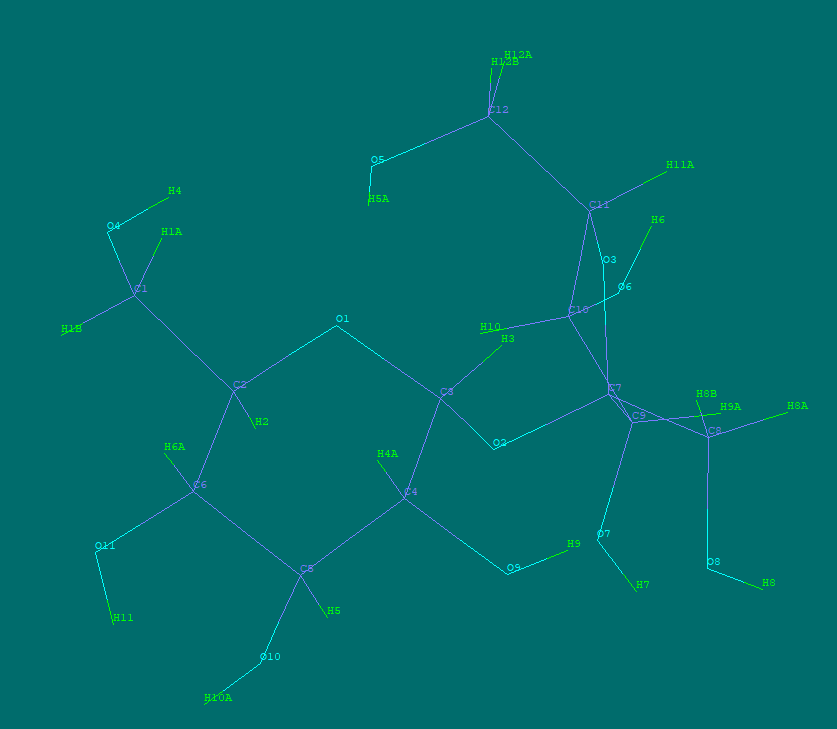
\includegraphics[width=0.8\linewidth]{Molecule_1}
	\caption{Смоделированная структура сахарозы, вид (а)}
	\label{fig:sucrose_a}
\end{figure}

\begin{figure}[H]
	\centering
	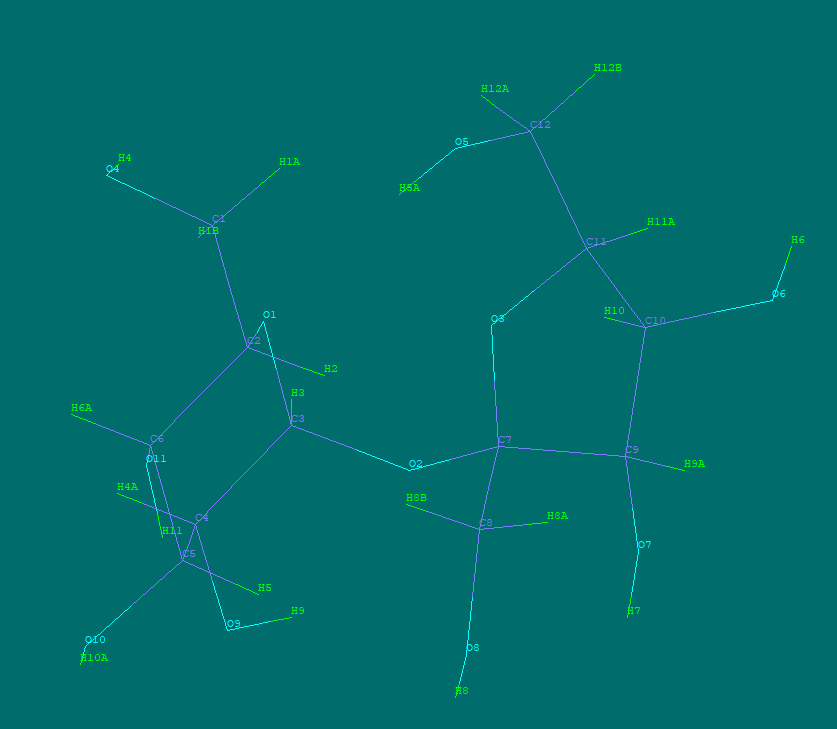
\includegraphics[width=0.8\linewidth]{Molecule_2}
	\caption{Смоделированная структура сахарозы, вид (b)}
	\label{fig:sucrose_b}
\end{figure}

\begin{figure}[H]
	\centering
	\includegraphics[width=0.6\linewidth]{log}
	\caption{К полученному $R$}
	\label{fig:log}
\end{figure}



\newpage

\begin{thebibliography}{1}
	\bibitem{Practicum}
	Рентгендифракционные методы изучения структуры монокристаллов, поликристаллических и аморфных материалов
\end{thebibliography}


\end{document}